% Figura cuerpo B2 (3.2.1): escalonamiento: por qué el nivel de precios es lento aunque cada precio cambie a menudo
\documentclass[tikz,border=3pt]{standalone}
\usepackage[T1]{fontenc}
\usepackage[utf8]{inputenc}
\usepackage{amsmath}
\usetikzlibrary{arrows.meta,calc,positioning}
\begin{document}
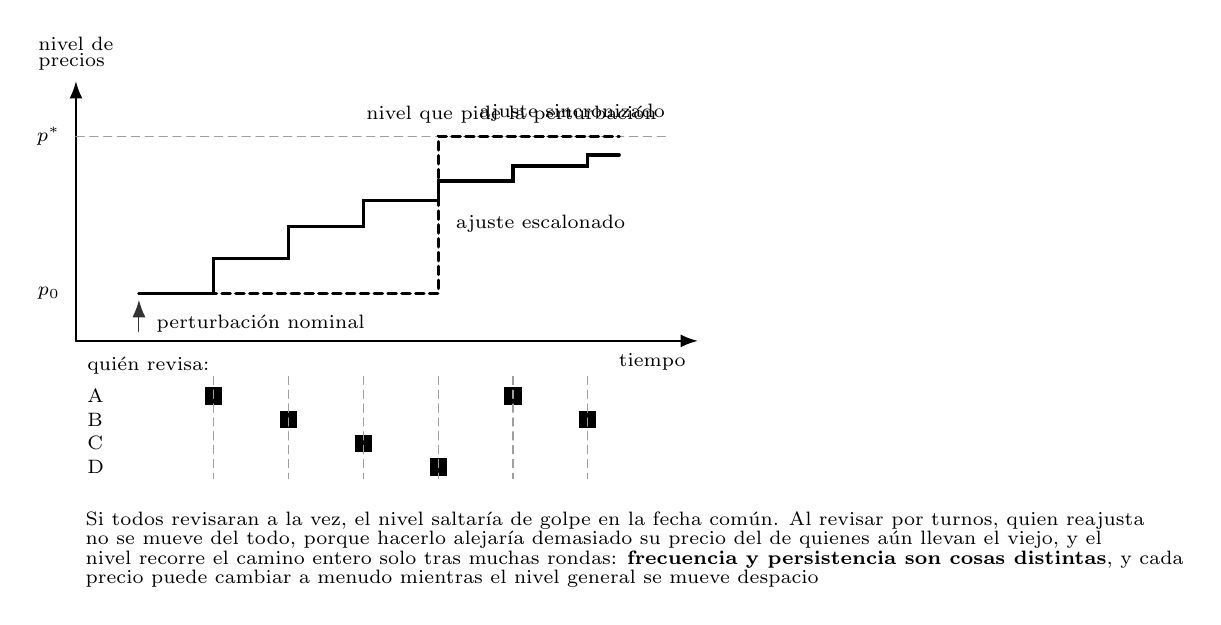
\begin{tikzpicture}[>={Latex[length=2.2mm]}, line cap=round, font=\footnotesize,
  eje/.style={->, thick},
  esc/.style={very thick},
  sinc/.style={very thick, densely dashed},
  guia/.style={densely dashed, gray!75}]

  \draw[eje] (0,0) -- (7.9,0) node[below left=1pt, font=\scriptsize]{tiempo};
  \draw[eje] (0,0) -- (0,3.3) node[above, font=\scriptsize, align=left]{nivel de\\[-2pt]precios};

  \draw[guia] (0,2.6) -- (7.5,2.6);
  \node[anchor=east, font=\scriptsize] at (-0.08,2.6) {$p^{*}$};
  \node[anchor=south east, font=\scriptsize] at (7.5,2.64) {nivel que pide la perturbación};
  \node[anchor=east, font=\scriptsize] at (-0.08,0.6) {$p_{0}$};

  % Ajuste sincronizado: todos revisan en la fecha común
  \draw[sinc] (0.8,0.6) -- (4.6,0.6) -- (4.6,2.6) -- (6.9,2.6);
  \node[anchor=south west, font=\scriptsize] at (5.0,2.66) {ajuste sincronizado};

  % Ajuste escalonado: por turnos
  \draw[esc] (0.8,0.60) -- (1.75,0.60) -- (1.75,1.05) -- (2.70,1.05) -- (2.70,1.45)
          -- (3.65,1.45) -- (3.65,1.78) -- (4.60,1.78) -- (4.60,2.03)
          -- (5.55,2.03) -- (5.55,2.22) -- (6.50,2.22) -- (6.50,2.36) -- (6.90,2.36);
  \node[anchor=north west, font=\scriptsize] at (4.70,1.72) {ajuste escalonado};

  \draw[->, gray!40!black] (0.8,0.12) -- (0.8,0.52);
  \node[anchor=west, font=\scriptsize] at (0.90,0.22) {perturbación nominal};

  % Calendario de turnos
  \node[anchor=west, font=\scriptsize] at (0.02,-0.32) {quién revisa:};
  \foreach \f/\y in {A/-0.70, B/-1.00, C/-1.30, D/-1.60}
    \node[anchor=west, font=\scriptsize] at (0.02,\y) {\f};
  \foreach \x/\y in {1.75/-0.70, 2.70/-1.00, 3.65/-1.30, 4.60/-1.60, 5.55/-0.70, 6.50/-1.00}
    \fill (\x-0.11,\y-0.11) rectangle (\x+0.11,\y+0.11);
  \foreach \x in {1.75,2.70,3.65,4.60,5.55,6.50} \draw[guia] (\x,-0.45) -- (\x,-1.75);

  \node[align=left, anchor=north west, font=\scriptsize] at (0,-2.05)
    {Si todos revisaran a la vez, el nivel saltaría de golpe en la fecha común. Al revisar por turnos, quien reajusta\\[-1pt]no se mueve del todo, porque hacerlo alejaría demasiado su precio del de quienes aún llevan el viejo, y el\\[-1pt]nivel recorre el camino entero solo tras muchas rondas: \textbf{frecuencia y persistencia son cosas distintas}, y cada\\[-1pt]precio puede cambiar a menudo mientras el nivel general se mueve despacio};
\end{tikzpicture}
\end{document}
